\documentclass[tikz,border=12pt]{standalone}
\usepackage[T1]{fontenc}
\usepackage{mathpazo}
\usepackage{amsmath,amssymb}
\usetikzlibrary{arrows.meta, positioning, calc, fit, decorations.pathreplacing, shadows.blur}

\definecolor{stblue}{HTML}{7B97AD}
\definecolor{rwgold}{HTML}{B8995E}
\definecolor{sage}{HTML}{7A9A7E}
\definecolor{dkbrown}{HTML}{3D3530}
\definecolor{wmgray}{HTML}{7B7067}
\definecolor{cream}{HTML}{F9F6F0}
\definecolor{border}{HTML}{D4C9B8}
\definecolor{terracotta}{HTML}{C47A6A}
\definecolor{lavender}{HTML}{907EA0}

\begin{document}
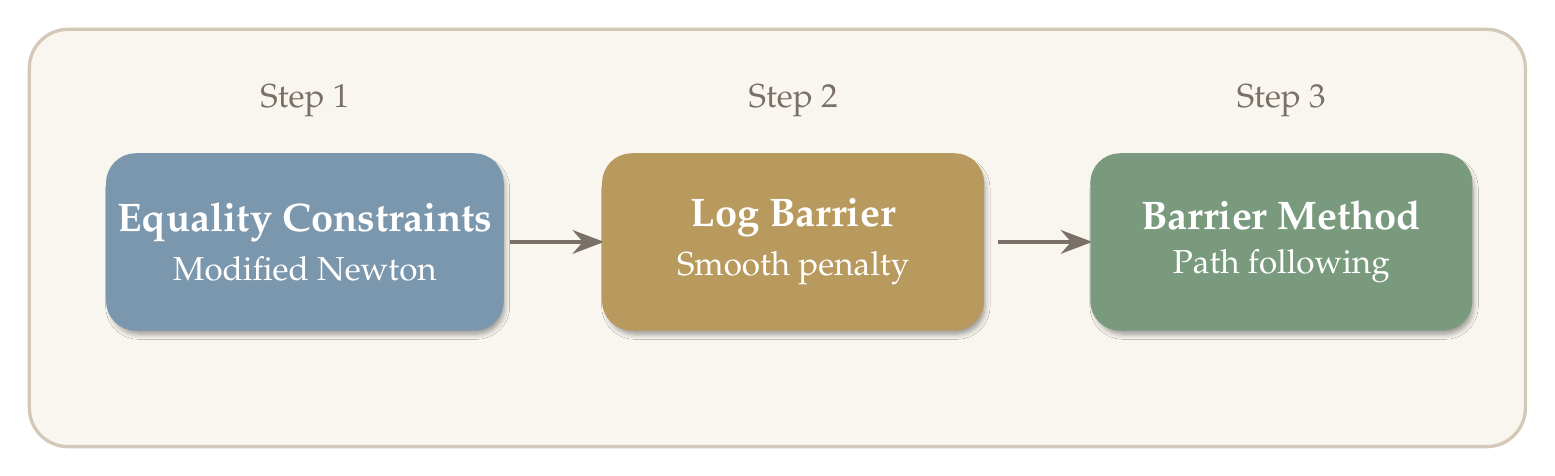
\begin{tikzpicture}[>={Stealth[length=4mm, width=3mm]}, line width=1.5pt]

% Background
\fill[cream, rounded corners=14pt] (-0.5,-0.8) rectangle (18.5,4.5);
\draw[border, line width=1.2pt, rounded corners=14pt] (-0.5,-0.8) rectangle (18.5,4.5);

% Box 1: Equality Constraints
\node[draw=stblue, line width=1.5pt, fill=stblue, rounded corners=10pt,
      minimum width=4.8cm, minimum height=2.2cm, align=center,
      blur shadow={shadow blur steps=5, shadow xshift=1pt, shadow yshift=-2pt}]
      (box1) at (3.0,1.8) {{\color{white}\textbf{\Large Equality Constraints}}\\[4pt]
      {\color{white!85}\large Modified Newton}};
\node[text=wmgray, font=\large] at (3.0,3.6) {Step 1};

% Arrow 1->2
\draw[wmgray, ->, line width=1.5pt] (5.6,1.8) -- (6.8,1.8);

% Box 2: Log Barrier
\node[draw=rwgold, line width=1.5pt, fill=rwgold, rounded corners=10pt,
      minimum width=4.8cm, minimum height=2.2cm, align=center,
      blur shadow={shadow blur steps=5, shadow xshift=1pt, shadow yshift=-2pt}]
      (box2) at (9.2,1.8) {{\color{white}\textbf{\Large Log Barrier}}\\[4pt]
      {\color{white!85}\large Smooth penalty}};
\node[text=wmgray, font=\large] at (9.2,3.6) {Step 2};

% Arrow 2->3
\draw[wmgray, ->, line width=1.5pt] (11.8,1.8) -- (13.0,1.8);

% Box 3: Barrier Method
\node[draw=sage, line width=1.5pt, fill=sage, rounded corners=10pt,
      minimum width=4.8cm, minimum height=2.2cm, align=center,
      blur shadow={shadow blur steps=5, shadow xshift=1pt, shadow yshift=-2pt}]
      (box3) at (15.4,1.8) {{\color{white}\textbf{\Large Barrier Method}}\\[4pt]
      {\color{white!85}\large Path following}};
\node[text=wmgray, font=\large] at (15.4,3.6) {Step 3};

\end{tikzpicture}
\end{document}
